% !TeX root = ../main.tex
\chapter{ATE Connections}
\label{chap:ATE}
\section{Overview}
	\noindent\textbf{On initial setup,} there are a few fixed connections that need to be made to the ATE:
	\begin{itemize}[noitemsep, topsep=0pt]
		\item Current Shunt: Connect this to a resistance standard for calibrations, or to a wire loop if not being used for current measurement
		\item $\pm15V$ Supply: Connect this to a split supply, draws less than 400mA under full load
		\item Network: Connect to the local test network
		\item SD Card must be configured once, but does not require any regular changes
		\item Jumpers: Install jumpers in J8-9, J12-13,  J19-20, JJ23-24, J30-31, J34-35, J41-42, and J45-J46 for normal operations.
	\end{itemize}

	\noindent\textbf{\\\\For every device under test:}
	\begin{itemize}[noitemsep, topsep=0pt]
		\item Channel 1, 2, 3, and 4 Power Supply Cables: These cables connect to each of the micro-D Power Supply I/O connectors on the rear of the PSC
		\item Tuning Boards: Tuning boards must be installed to match the loads being tested.
		\item DCCT Cable must be connected for every PSC. There are two cables - one for 4-Channel units, and another for 2-Channel units. 
	\end{itemize}
	
	\begin{figure}[H]
		\centering
		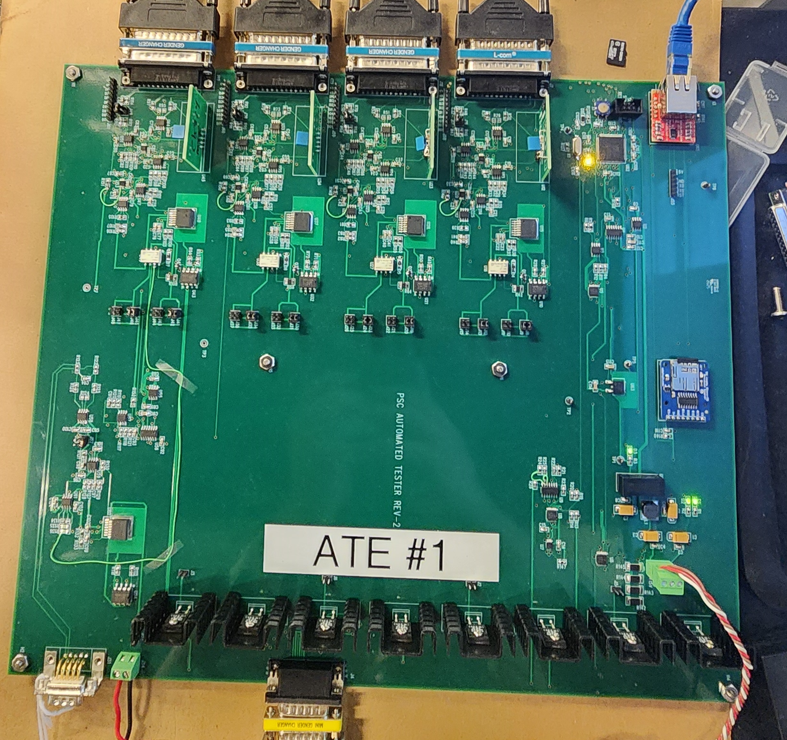
\includegraphics[width=6in]{Pictures/ATE_Cropped}
		\caption{ATE \#1}
	\end{figure}

	\subsection{ATE Test Rack at NSLS-II}
		\begin{figure}[H]
			\centering
			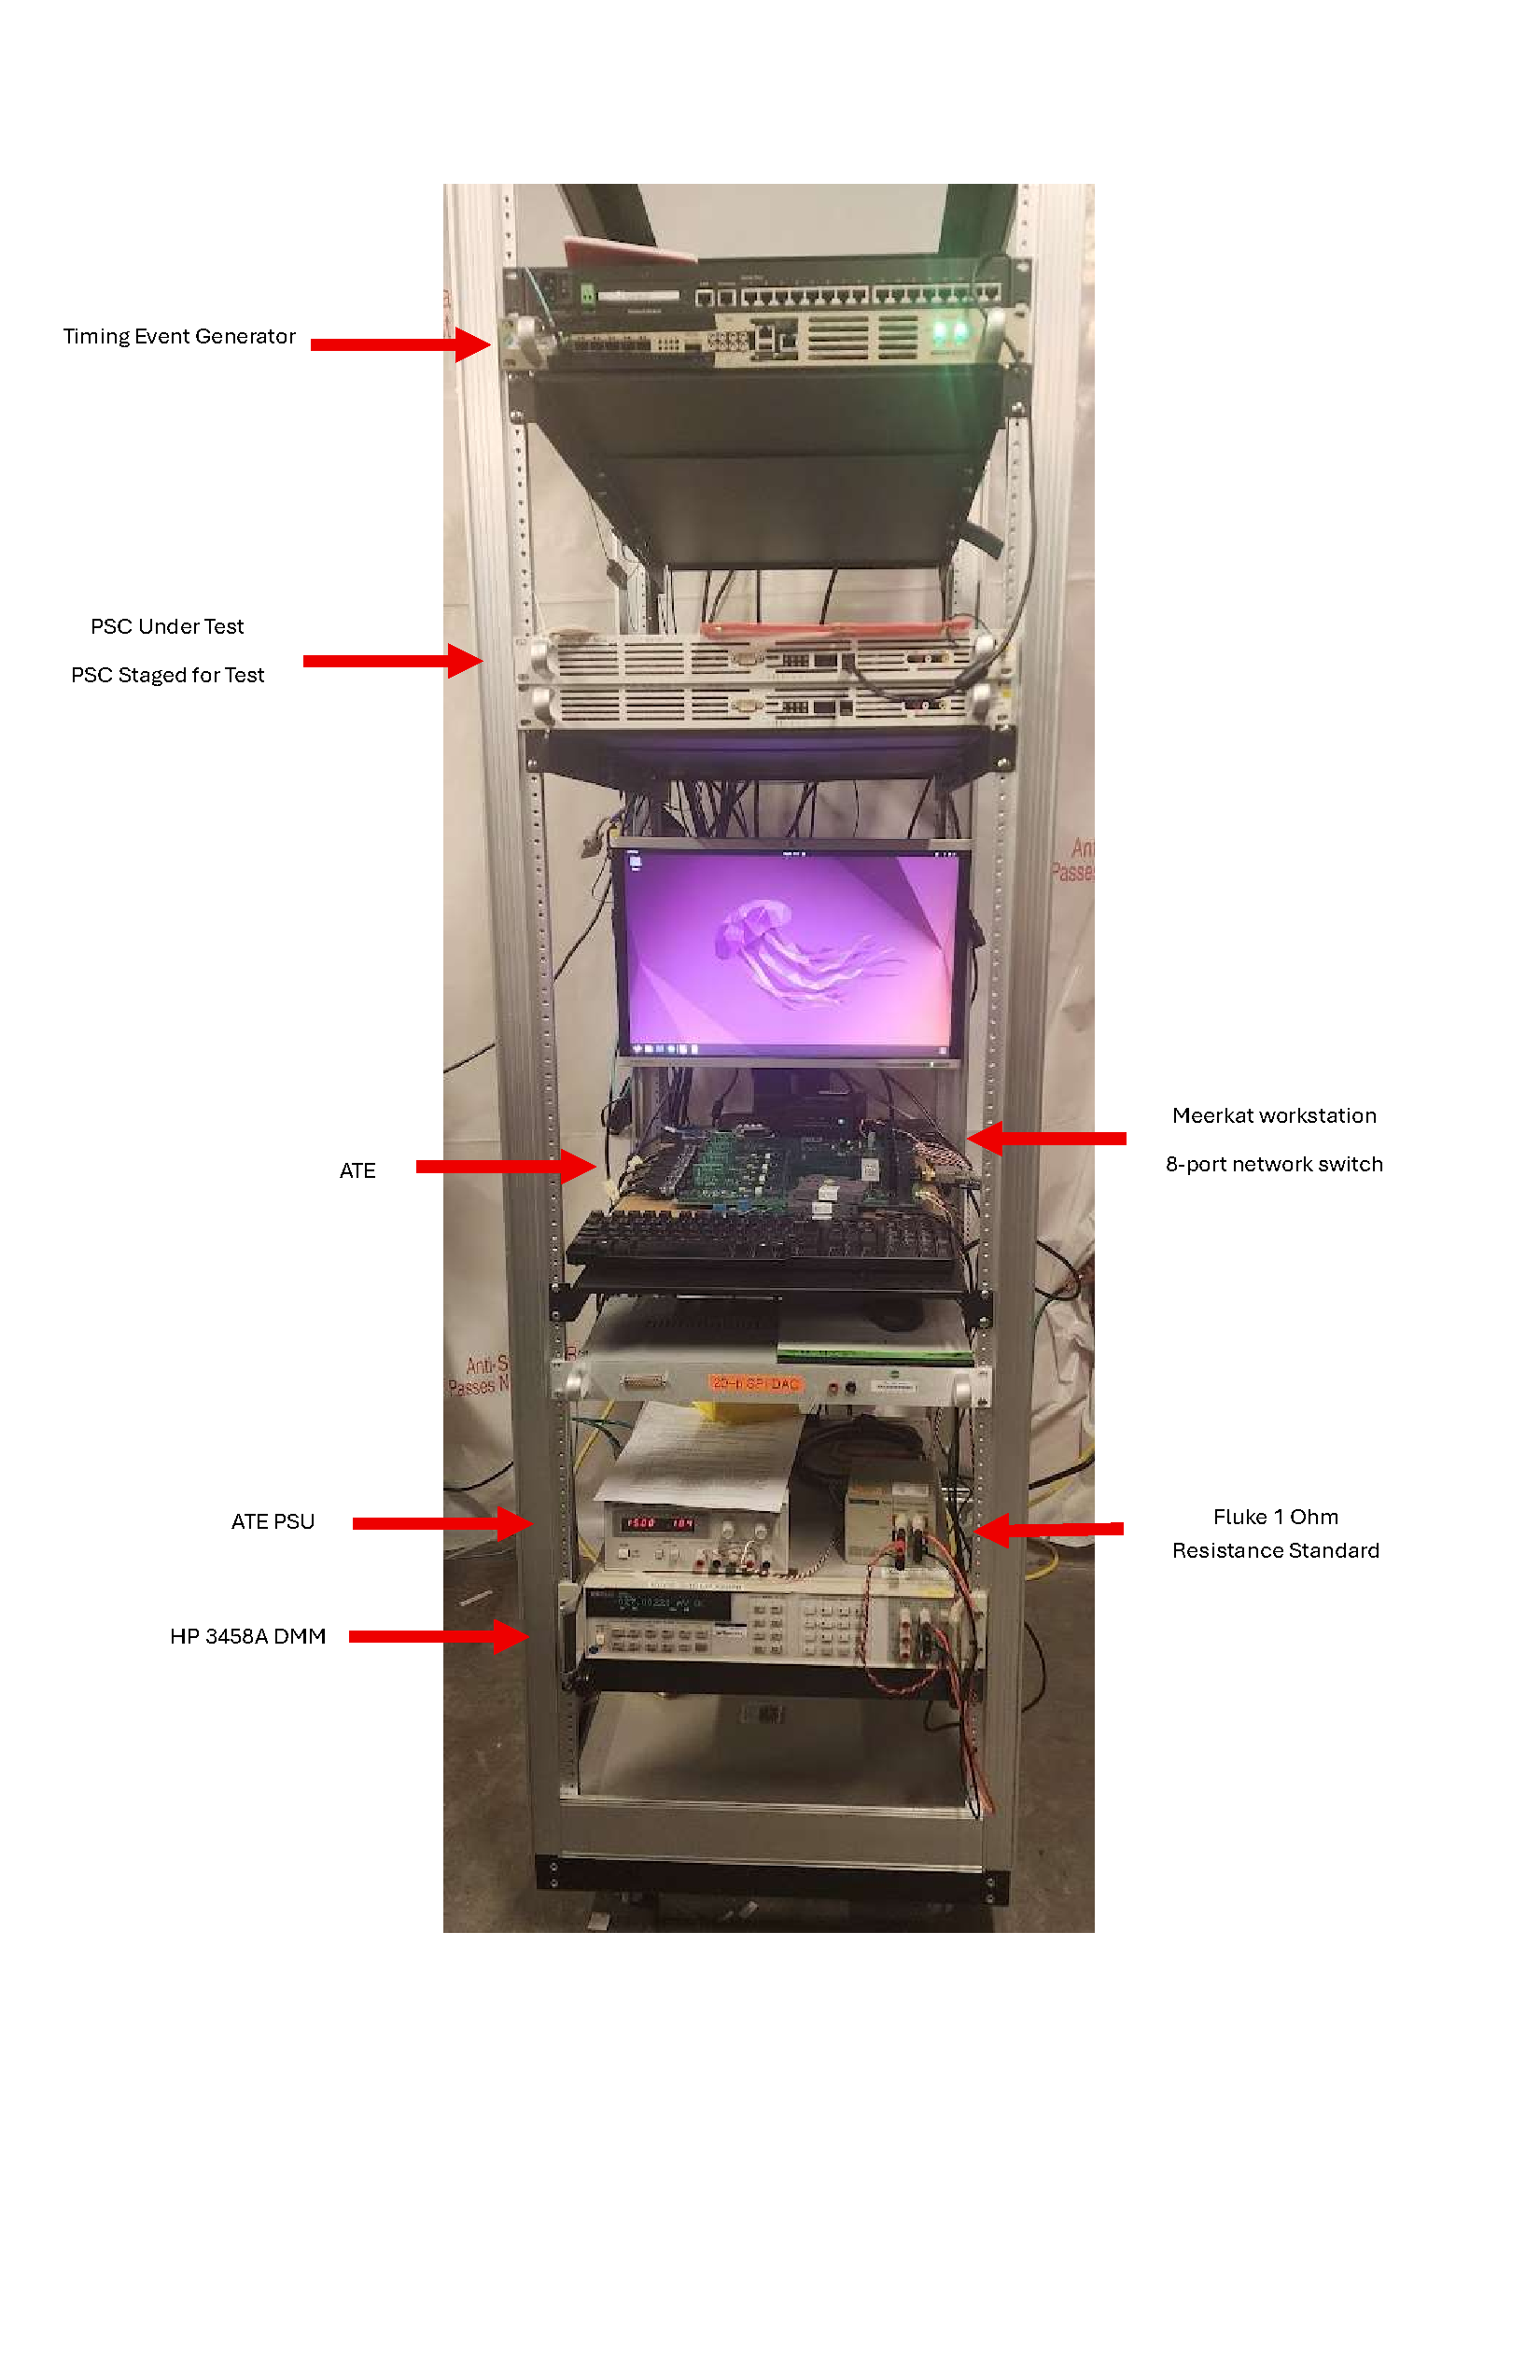
\includegraphics[
			width=5.5in,
			%height=0.85\textwidth,
			keepaspectratio
			]{Pictures/TestRackAnnotated}
		\end{figure}
		
\section{Connections}
	\begin{figure}[H]
	\centering
	\resizebox{\textwidth}{!}{%
		\begin{tikzpicture}[
			>=latex,
			chassis/.style={
				draw,
				rectangle,
				line width=0.8pt,
				align=center
			},
			module/.style={
				draw,
				rectangle,
				minimum width=2.5cm,
				minimum height=0.75cm,
				align=center,
				font=\small
			},
			block/.style={
				draw,
				rectangle,
				minimum width=3.0cm,
				minimum height=1.0cm,
				align=center,
				font=\small
			},
			shuntblock/.style={
				draw,
				rectangle,
				minimum width=4cm,
				minimum height=1.4cm,
				align=center,
				font=\small
			}
			]
			
			% ==================================================
			% PSC CHASSIS
			% ==================================================
			\node[
			chassis,
			minimum width=3.4cm,
			minimum height=6.6cm
			] (psc) at (0,0) {};
			
			\node[font=\Large\bfseries] at (0,2.75) {PSC};
			
			\node[module] (dcct) at (0,1.7) {DCCT};
			\node[module] (ch1)  at (0,0.7) {CH1};
			\node[module] (ch2)  at (0,-0.3) {CH2};
			\node[module] (ch3)  at (0,-1.3) {CH3};
			\node[module] (ch4)  at (0,-2.3) {CH4};
			
			% ==================================================
			% ATE CHASSIS
			% ==================================================
			\node[
			chassis,
			minimum width=3.8cm,
			minimum height=13.5cm
			] (ate) at (6.0,-2.5) {};
			
			\node[font=\Large\bfseries] at (6.0,3.4) {ATE};
			
			\node[module] (ate_dcct) at (6.0,1.7) {DCCT};
			\node[module] (ate_ch1)  at (6.0,0.7) {CH1};
			\node[module] (ate_ch2)  at (6.0,-0.3) {CH2};
			\node[module] (ate_ch3)  at (6.0,-1.3) {CH3};
			\node[module] (ate_ch4)  at (6.0,-2.3) {CH4};
			
			\node[module] (ate_pwr) at (6.0,-4.0) {$\pm15$ V};
			\node[module] (ate_net) at (6.0,-5.4) {Network};
			
			% ATE Current Shunt block inside chassis
			\node[
			shuntblock,
			minimum width=3.2cm,
			minimum height=1.8cm
			] (ate_shunt) at (6.0,-7.4)
			{
				ATE Current Shunt\\
				Terminal Block
			};
			
			% ==================================================
			% PSC -> ATE CONNECTIONS
			% ==================================================
			\draw[->] (dcct.east) -- (ate_dcct.west);
			\draw[->] (ch1.east)  -- (ate_ch1.west);
			\draw[->] (ch2.east)  -- (ate_ch2.west);
			\draw[->] (ch3.east)  -- (ate_ch3.west);
			\draw[->] (ch4.east)  -- (ate_ch4.west);
			
			% ==================================================
			% POWER SUPPLY + NETWORK SWITCH
			% ==================================================
			\node[block] (supply) at (0,-4.0)
			{
				$\pm15$ V\\
				Power Supply
			};
			
			\node[block] (switch) at (0,-5.4)
			{
				Network\\
				Switch
			};
			
			\draw[->] (supply.east) -- (ate_pwr.west);
			\draw[->] (switch.east) -- (ate_net.west);
			
			% ==================================================
			% RESISTANCE STANDARD
			% ==================================================
			\node[
			block,
			minimum width=6cm,
			minimum height=4cm,
			inner sep=12pt
			] (resistor) at (14.0,-7.4)
			{
				4-Terminal\\[6pt]
				Resistance Standard\\[6pt]
				\quad Fluke 742A-1 or equivalent\quad\mbox{}\\[6pt]
				1 Ohm
			};
			
			% ==================================================
			% DMM
			% ==================================================
			\node[
			block,
			minimum width=6cm,
			minimum height=3.6cm
			] (dmm) at (22.0,-7.4)
			{
				DMM\\[10pt]
				HP 3458A or equivalent
			};
			
			% GPIB block INSIDE DMM
			\node[
			draw,
			rectangle,
			minimum width=3.2cm,
			minimum height=0.8cm,
			font=\small
			] (gpib) at ($(dmm.south)+(0,0.4)$)
			{GPIB};
			
			% ==================================================
			% PROLOGIX
			% ==================================================
			\node[
			draw,
			rectangle,
			minimum width=5cm,
			minimum height=1.2cm,
			font=\small
			] (prologix) at ($(dmm.south)+(0,-2.0)$)
			{Prologix GPIB Adapter};
			
			\draw[->, thick] (gpib.south) -- (prologix.north);
			
			% ==================================================
			% SIDE LABELS
			% ==================================================
			\node[
			draw,
			rotate=90,
			fill=white,
			inner sep=4pt
			]
			at ($(resistor.west)+(0.3,0)$)
			{CURRENT};
			
			\node[
			draw,
			rotate=90,
			fill=white,
			inner sep=4pt
			]
			at ($(resistor.east)+(-0.3,0)$)
			{SENSE};
			
			\node[
			draw,
			rotate=90,
			fill=white,
			inner sep=4pt
			]
			at ($(dmm.west)+(0.35,0)$)
			{Input};
			
			% ==================================================
			% MEASUREMENT CHAIN CONNECTIONS
			% ==================================================
			\draw[->, thick] (ate_shunt.east) -- (resistor.west);
			\draw[->, thick] (resistor.east) -- (dmm.west);
			
		\end{tikzpicture}%
	}
	\caption{ATE Connection Block Diagram}
	\label{fig:psc_ate_block_diagram}
\end{figure}

\begin{figure}[H]
	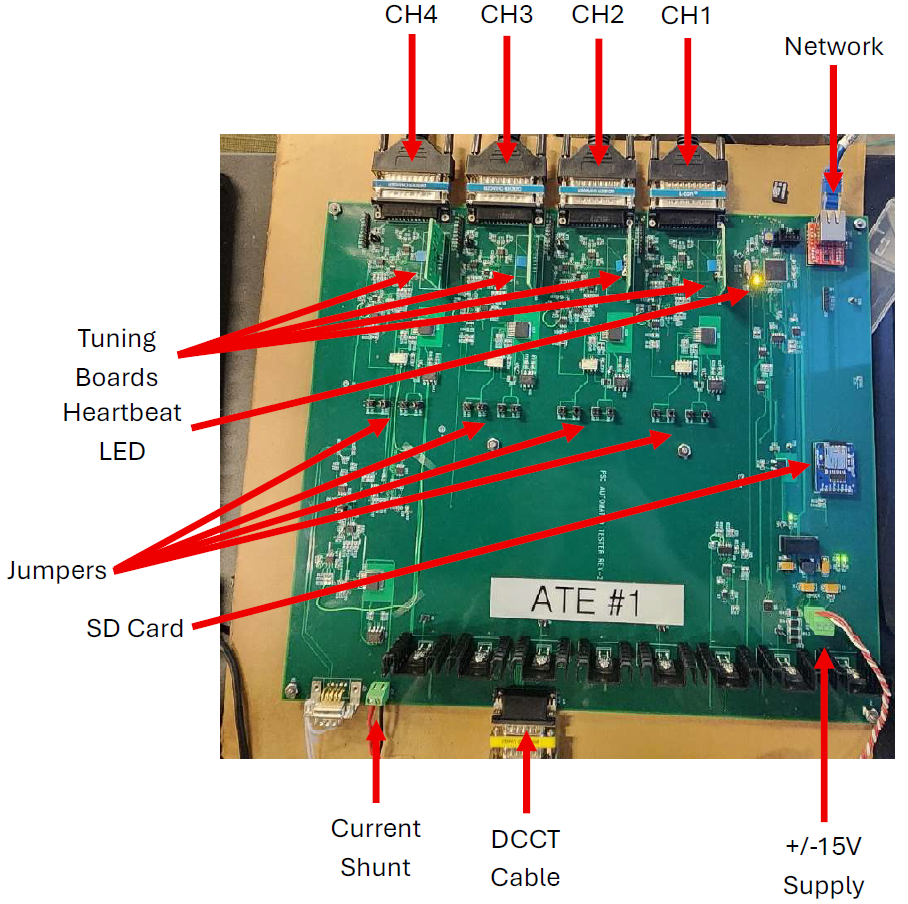
\includegraphics[width=\textwidth]{Pictures/ATE_Annotated}
	\caption{Annotated ATE Board}
\end{figure}

\newpage
\subsection{Current Measurement Loop/DMM Connection}
The DMM is connected to the workstation via a GPIB adapter from Prologix. These are available in both USB and Ethernet forms.\\\\
%
\begin{center}
	\setlength{\fboxrule}{1.5pt}
	\setlength{\fboxsep}{6pt}
	\fbox{
		\parbox{0.9\textwidth}{
			\textbf{If the DMM/Resistance standard is not used, a jumper must be connected across this terminal block on the ATE if CALDAC is to be used!}
		}
	}
\end{center}

\begin{figure}[H]
	\centering
		\resizebox{0.75\textwidth}{!}{%
		\begin{tikzpicture}[
			>=latex,
			chassis/.style={
				draw,
				rectangle,
				line width=0.8pt,
				align=center
			},
			module/.style={
				draw,
				rectangle,
				minimum width=2.5cm,
				minimum height=0.75cm,
				align=center,
				font=\small
			},
			block/.style={
				draw,
				rectangle,
				minimum width=3.0cm,
				minimum height=1.0cm,
				align=center,
				font=\small
			},
			shuntblock/.style={
				draw,
				rectangle,
				minimum width=4cm,
				minimum height=1.4cm,
				align=center,
				font=\small
			}
			]
			
			% ==================================================
			% ATE CHASSIS
			% ==================================================
			\node[
			chassis,
			minimum width=3.8cm,   % restored original width
			minimum height=4.8cm
			] (ate) at (6.0,-7.4) {};
			
			\node[font=\Large\bfseries] at (6.0,-5.8) {ATE};
			
			% ATE Current Shunt block inside chassis
			\node[
			shuntblock,
			minimum width=3.2cm,   % restored original inner width
			minimum height=1.2cm
			] (ate_shunt) at (6.0,-7.4)   % moved up for horizontal arrow
			{
				ATE Current Shunt\\
				Terminal Block
			};
			
			% ==================================================
			% RESISTANCE STANDARD
			% ==================================================
			\node[
			block,
			minimum width=6cm,
			minimum height=4cm,
			inner sep=12pt
			] (resistor) at (14.0,-7.4)
			{
				4-Terminal\\[6pt]
				Resistance Standard\\[6pt]
				\quad Fluke 742A-1 or equivalent\quad\mbox{}\\[6pt]
				1 Ohm
			};
			
			% ==================================================
			% DMM
			% ==================================================
			\node[
			block,
			minimum width=6cm,
			minimum height=3.6cm
			] (dmm) at (22.0,-7.4)
			{
				DMM\\[10pt]
				HP 3458A or equivalent
			};
			
			% GPIB block INSIDE DMM
			\node[
			draw,
			rectangle,
			minimum width=3.2cm,
			minimum height=0.8cm,
			font=\small
			] (gpib) at ($(dmm.south)+(0,0.4)$)
			{GPIB};
			
			% ==================================================
			% PROLOGIX
			% ==================================================
			\node[
			draw,
			rectangle,
			minimum width=5cm,
			minimum height=1.2cm,
			font=\small
			] (prologix) at ($(dmm.south)+(0,-2.0)$)
			{Prologix GPIB Adapter};
			
			\draw[->, thick] (gpib.south) -- (prologix.north);
			
			% ==================================================
			% SIDE LABELS
			% ==================================================
			\node[
			draw,
			rotate=90,
			fill=white,
			inner sep=4pt
			]
			at ($(resistor.west)+(0.3,0)$)
			{CURRENT};
			
			\node[
			draw,
			rotate=90,
			fill=white,
			inner sep=4pt
			]
			at ($(resistor.east)+(-0.3,0)$)
			{SENSE};
			
			\node[
			draw,
			rotate=90,
			fill=white,
			inner sep=4pt
			]
			at ($(dmm.west)+(0.35,0)$)
			{Input};
			
			% ==================================================
			% MEASUREMENT CHAIN CONNECTIONS
			% ==================================================
			\draw[->, thick] (ate_shunt.east) -- (resistor.west);
			\draw[->, thick] (resistor.east) -- (dmm.west);
			
		\end{tikzpicture}%
	}
	\caption{ATE $\rightarrow$ DMM Current Loop}
\end{figure}

\subsection{Tuning Boards}
	The ATE contains four Tuning Board sockets, one per channel. Tuning boards must be installed for each channel under test.\\\\ The tuning boards must be matched to the PSC configuration. Each channel's tuning board must be installed as a counterpart to the burdens and comps installed in the PSC, as it simulates the response of the magnet load.
	\begin{figure}[H]
		\centering
		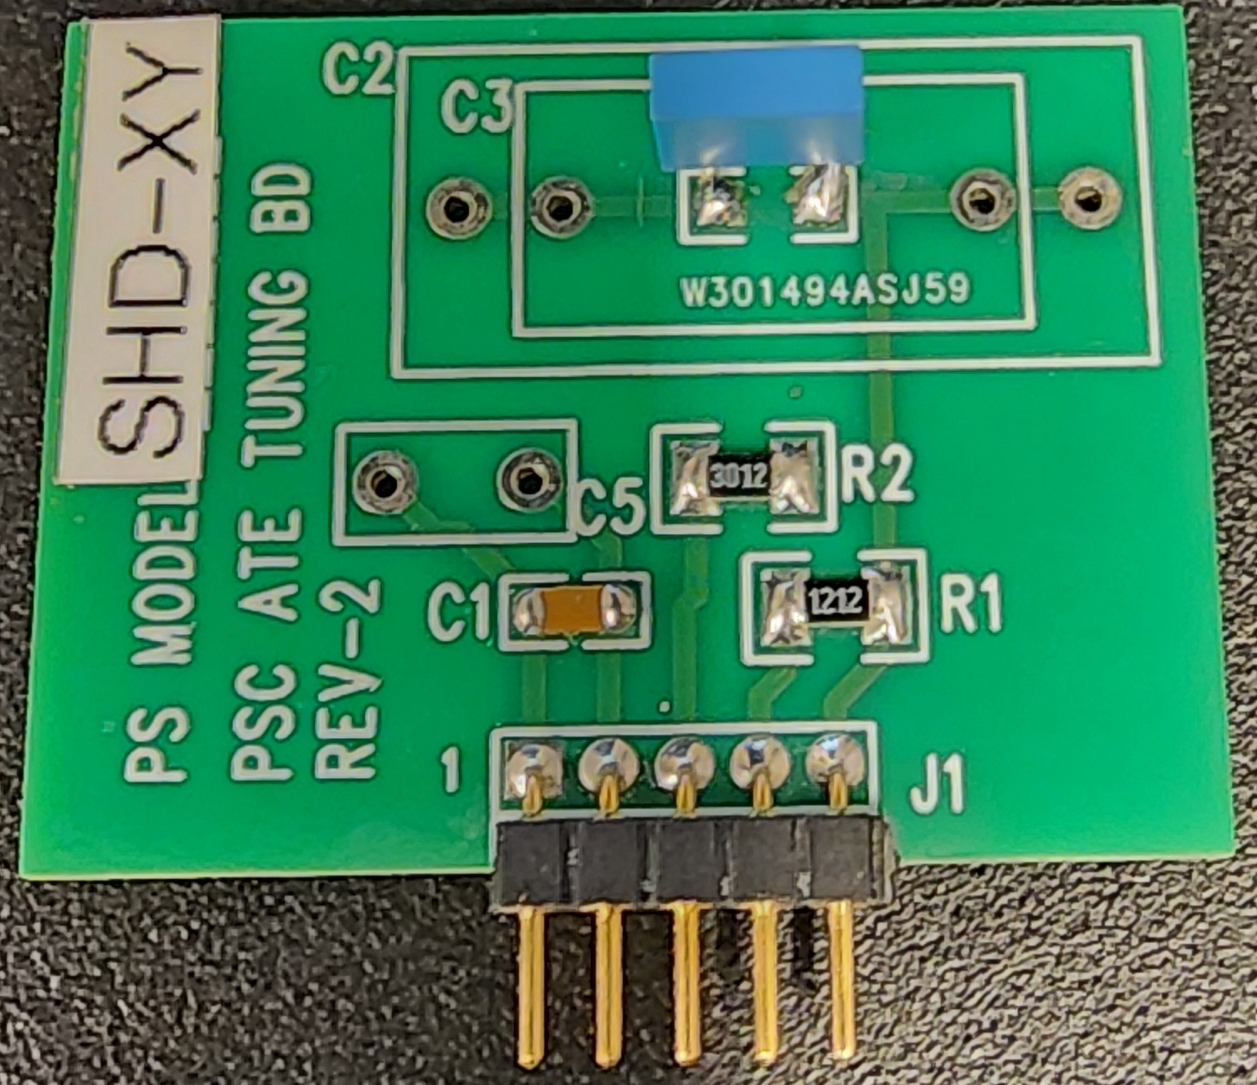
\includegraphics[width=3in]{Pictures/Tuning_Board}
		\caption{ATE Tuning Board for the ALSu SHD-XY Magnet}
	\end{figure}